\documentclass[c_worksheet.tex]{subfiles}

\begin{document}
	
\chapter{Fortgeschrittene Aufgaben}

In diesem Teil gibt es Aufgaben die schon etwas schwieriger sind. Hier kommen sowohl \emph{Pointer}, \emph{Arrays} als auch \emph{Structs} zum Einsatz.


\section{Minimum}


Schreibe eine \emph{Funktion}, die ein \emph{Array} von Zahlen übergeben bekommt, und das kleinste Element zurück gibt. \\

Wie kannst du die Funktion so abändern, dass du anstatt dem Minimum, das Maximum berechnest. 



\section{Mittelwert}

Schreibe eine \emph{Funktion}, die ein \emph{Array} von Zahlen übergeben bekommt, und den Mittelwert dieser berechnet.



\section{Schnitt zweier Rechtecke}

Definiere ein \emph{struct} \textbf{point2D}, welches einen Punkt im 2-dimensionalen Raum repräsentieren soll. Dazu brauch das \emph{struct} einen X- und einen Y-Wert. Nutze dafür einfache \emph{Interger} Variablen.

Dann erstelle eine weitere Struktur \textbf{rectangle}, die ein Rechteck darstellen soll. Dafür braucht es lediglich zwei Variablen vom \emph{Typ} \textbf{point2D}. Den Punkt ganz oben links, und den unten rechts.

Schreibe eine Funktion, welche die Schnittfläche zweier Rechtecke berechnet.\\

\textbf{Bonus:} Schreibe eine Funktion, die als Rückgabe die Schnittfläche als Rechteck liefert und einen \textbf{null} \emph{Pointer}, wenn der Schnitt leer ist.



\section{Rekursion} 


Eine Rekursive Funktion, ist eine Funktion die sich selbst wieder aufruft.

Die Fakultät ist dabei rekursiv wie folgt definiert:

\begin{align*}
	Fak(n) &= n * Fak(n-1) \\
	Fak(0) &= 1
\end{align*}

Implementiere die Fakultät mit einer rekursive Funktion in \textbf{C}.



\section{Sliding Window} 

Das Sliding Window Prinzip ist auch in der Programmierwelt relativ bekannt und kommt des öfteren zum Einsatz.

Dabei hat man ein Fenster einer gewissen Größe \(k\) das z.B. durch ein \emph{Array} ``slidet''. Für den Algorithmus sind dann immer nur die Werte innerhalb des Fensters von Bedeutung.

\begin{figure}[h]
\center
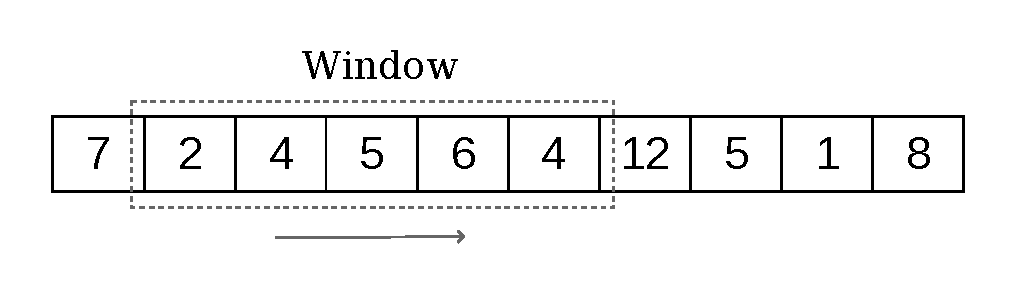
\includegraphics[width=0.8\textwidth]{Grafiken/Aufgaben/slidingWindow} 
\end{figure}

Schreibe eine Funktion, die ein \emph{Array} von Zahlenwerten nimmt und mit einem Sliding Window der Größe \textbf{5} durch das Array läuft. Am Ende gibt die Funktion auch wieder ein \emph{Array} zurück.

Innerhalb des Fensters werden alle Werte aufaddiert und durch \textbf{5} geteilt. Das ist dann der neue Wert in der Mitte des Fensters. Dabei sollen allerdings nicht alle Werte gleichstark gewichtet werden. Werte weiter entfernt vom Zentrum des Fensters, sollen am wenigsten stark ins Gewicht fallen. Das Zentrum selbst am meisten.\\

Das erreichst du mit so genannten \emph{Gewichtungsfaktoren}. Das ganze könnte (entlang des Beispiels) z.B so aussehen:

\begin{align*}
	zentrum &= \frac{0.5 * \textbf{2} + 0.75 * \textbf{4} + 1.0 * \textbf{5} + 0.75 * \textbf{6} + 0.5 * \textbf{4}}{5} \\
	zentrum &= 3.1
\end{align*}

Das ist übrigens genau, was beim so genannten \emph{Gauß-Filter} passiert, nur dort eben in 2 Dimensionen.

Du musst aufpassen, was an den Grenzen des Arrays passiert. Überlege dir was du dort tust. Ob du dort vielleicht nur 3 Werte benutzt, oder ob du eine Art ``Wrap-around'' machst, also so, als wäre das \emph{Array} ein Ring und die letzten Werte werden mit berücksichtigt. \\

\textbf{Bonus:} Ändere die Funktion so ab, dass sie noch eine Fenster Größe \(k\) als Parameter annimmt und das ganze dementsprechend durchführt.



\section{Stack}

Ein Stack ist eine, beim Programmieren immer wieder benutzte Datenstruktur. Im Prinzip ist es ein Stapel, wie auch der Kartenstapel beim Mau Mau. Man kommt immer nur an das oberste Elemente, nicht aber an die darunter.

Man kann dann Elemente oben auf den Stack legen, und auch immer nur das oberste wieder herunter nehmen.

Ein Stack hat nur zwei Operationen

\begin{itemize}
	\item \textbf{push} \\
	Legt ein neues Element oben auf den Stack
	\item \textbf{pop} \\
	Holt das oberste Element vom Stack runter
\end{itemize}

Du sollst nun so ein Stack mittels eines \emph{Structs} und eines \emph{Arrays} realisieren. 

Das \emph{struct} sollte etwa wie folgt aussehen

\begin{figure}[h]
\center
\begin{tabular}{ c | l }
\textbf{Name} & \textbf{Bedeutung} \\
\hline
data      & Ein Pointer auf das eigentliche Datenarray \\
size      & Die aktuelle Größe des Stacks \\
capacity  & Die aktuelle Kapazität des Arrays \\
\end{tabular}
\end{figure}

Mit Kapazität ist gemeint, wie groß das Array wirklich ist, also wie viel reinpasst. Die Größe gibt an, wie weit dieses Array gefüllt ist. Wächst der Stack über die Kapazität hinaus, muss das Array vergrößert werden.

Überlege dir, wie du das sinnvoll implementieren kannst. Überlege dir auch, ob es sinnvoll ist, dass Array immer nur um ein Element zu vergrößern, oder ob es vielleicht sinnvoller ist, das ganze um größere Stücke zu vergrößern. \\

\textbf{Bonus:} Füge dem Stack ein weiteres Attribut hinzu, das angibt um wie viel das Array jedes mal vergrößert werden soll.



\section{Reisetagebuch}

In dieser Aufgabe sollst du zwei Strukturen definieren.

Einmal die Struktur ``Reiseziel''. Diese hat folgende \emph{Attribute}

\begin{figure}[h]
\center
\begin{tabular}{ c | l }
\textbf{Name}     & \textbf{Bedeutung} \\
\hline
name     & Name des Reiseziels \\
distance & Entfernung des Reiseziels \\
country  & Der Name des Landes, in dem das Reiseziel liegt \\
\end{tabular}
\caption{Reiseziel} 
\end{figure}

Max führt ein Tagebuch über alle Reisen die er in seinem Leben schon gemacht hat. In Diesem Tagebuch schreibt er all seine Reisen in Form der Reiseziele auf.

Lege eine Struktur Reiseziel an, welche folgende \emph{Attribute} hat.

\begin{figure}[h]
\center
\begin{tabular}{ c | l }
\textbf{Name} & \textbf{Bedeutung} \\
\hline
owner  & Name des Reisetagebuchinhabers \\
journeyTargets & Liste aller besuchten Reiseziele \\
\end{tabular}
\caption{Reisetagebuch} 
\end{figure}

Lege ein paar Reiseziele an und ein Reisetagebuch, in welches du die Reiseziele einträgst. Schreibe dazu eine Funktion, die ein Reiseziel einem Reisetagebuch hinzufügt. Damit die Änderungen auch persistent sind, ist es wichtig, dass du die \emph{structs} als \emph{Referenz}, bzw per \emph{Pointer} übergibst.

\begin{lstlisting}
void addTarget(struct reisetagebuch* diary, struct reiseziel* target){
	// Code
}
\end{lstlisting}

Damit kannst du dann ganz leicht viele Reiseziele in das Reisetagebuch einfügen.

In solchen Situationen muss man oft \emph{Pointer} benutzen, da sonst die Funktion eine lokale Kopie der Parameter erstellt, und nicht auf dem ``Original'' arbeitet.

Schreibe folgende Funktionen

\begin{itemize}
	\item \textbf{distanceTraveled} \\
	Berechnet zu einem Reisetagebuch die zurückgelegte Distanz und gibt diese zurück
	\item \textbf{hasVisitedCountry} \\
	Überprüft zu einem Reisetagebuch und einem Land, ob die Person schon einmal dorthin gereist ist
	\item \textbf{visitedTargets} \\
	Gibt zu einem Reisetagebuch ein \emph{Array} mit den Namen aller besuchten Reiseziele zurück
	\item \textbf{visitedCountries} \\
	Gibt zu einem Reisetagebuch ein \emph{Array} mit allen Ländern zurück, die bisher bereist wurden
	\item \textbf{whoTravelledFurther} \\
	Nimmt zwei Reisetagebücher und gibt den Namen der Person, die bisher weiter gereist ist zurück
	\item \textbf{whoTravelledMoreCountires} \\
	Nimmt zwei Reisetagebücher und gibt den Namen der Person, die bisher mehr \textbf{verschiedene} Länder bereist hat zurück
	\item \textbf{numberOfTravelledCountires} \\
	Nimmt ein Reisetagebuch und gibt die Anzahl der bereisten Länder zurück 
\end{itemize}

\end{document}